\documentclass[tikz,border=10pt]{standalone}
\usetikzlibrary{arrows.meta,positioning,shapes.geometric}
\usepackage{xcolor}
\pagecolor{white}
\begin{document}
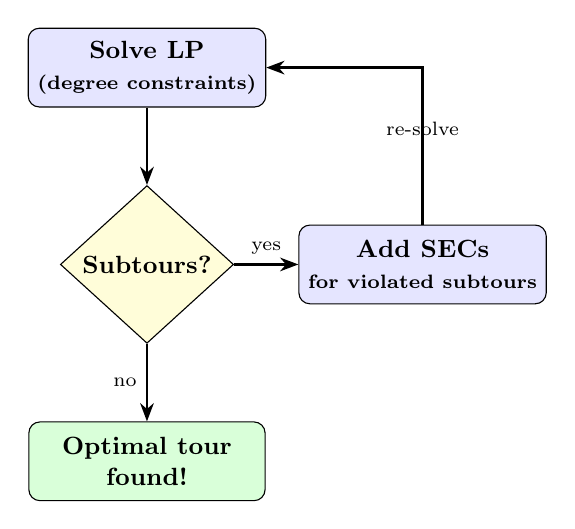
\begin{tikzpicture}[
  box/.style={draw, rounded corners, fill=blue!10, minimum width=3cm,
              minimum height=1cm, font=\small\bfseries, align=center},
  decision/.style={draw, diamond, fill=yellow!15, minimum width=2.2cm,
                   minimum height=1.5cm, font=\small\bfseries, align=center,
                   inner sep=1pt},
  arr/.style={-{Stealth}, thick},
  lbl/.style={font=\scriptsize, midway},
]
  \node[box] (solve) at (0, 0) {Solve LP\\{\scriptsize(degree constraints)}};
  \node[decision] (check) at (0, -2.5) {Subtours?};
  \node[box] (add) at (3.5, -2.5) {Add SECs\\{\scriptsize for violated subtours}};
  \node[box, fill=green!15] (done) at (0, -5) {Optimal tour\\found!};

  \draw[arr] (solve) -- (check);
  \draw[arr] (check) -- node[lbl, left] {no} (done);
  \draw[arr] (check) -- node[lbl, above] {yes} (add);
  \draw[arr] (add) |- node[lbl, above, pos=0.25] {re-solve} (solve);
\end{tikzpicture}
\end{document}
